%%%%%%%%%%%%%%%%%%%%%%%%%%%%%%%%%%%%%%%%%
% Kieker Analysis Component
% 
% $Date$
% $Rev$:
% $Author$


\chapter{\KiekerAnalysisPart{} Component}\label{chap:componentsAnalysis}

\NOTIFYBOX{The Java sources of this chapter can also be found in the %
\file{\customComponentsBookstoreApplicationDirDistro{}/} directory of the %
binary release.}

\section{Analysis Controller}\label{sec:analysis:controller}

An analysis with \KiekerAnalysisPart{} is set up and executed employing %
the class \class{AnalysisController}. %
\KiekerAnalysisPart{} requires a monitoring log reader %
(Section~\ref{sec:analysis:reader}) and at least %
one monitoring record consumer plugin (Section~\ref{sec:analysis:consumer}). %
In addition to the monitoring record consumer plugin, %
other analysis plugins can be registered. %
Figure~\ref{fig:analysisController:classdiagram} shows the class diagram %
with the important \KiekerAnalysisPart{} classes and their relationship. %

\begin{figure}[h]\centering
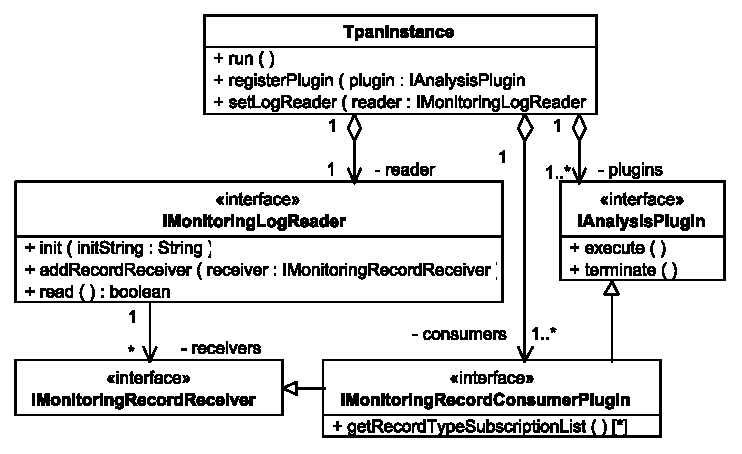
\includegraphics[scale=0.7]{images/kieker_TpanInstance}
\caption{\TODO{update}}
\label{fig:analysisController:classdiagram}
\end{figure}

\noindent Setting up and running an analysis with \KiekerAnalysisPart{} requires the %
following steps to be performed, as described in Section~\ref{sec:example:analysis} already:\\

\begin{compactenum}
\item Creating an instance of the \class{AnalysisController} class
\item Creating registering the monitoring log reader (\method{setLogReader}) as %
well as the monitoring record consumers and other analysis plugins (\method{registerPlugin}).
\item Starting the analysis instance (\method{run}).
\end{compactenum}

\

\noindent In the following Sections~\ref{sec:analysis:reader} and~\ref{sec:analysis:consumer}, %
we will create a custom monitoring log reader \class{MyPipeReader} and a %
monitoring record consumer plugin \class{MyResponseTimeConsumer}. %
\noindent The following Listing~\ref{listing:AnalysisController} shows how to create and run an analysis %
with these custom components:

\setJavaCodeListing
\lstinputlisting[caption=Starter.java,label=listing:AnalysisController,firstline=25, lastline=32, firstnumber=25]	{\customComponentsBookstoreApplicationDir/src/bookstoreApplication/Starter.java}

\section{Monitoring Log Readers}\label{sec:analysis:reader}

% Warning-tag for the reader-writer-thing
The monitoring log readers are the direct counterpart to the monitoring log writers. While a writer gets a record and writes it into files or somewhere else, the reader takes the written data and converts it into a suitable instance of \class{IMonitoringRecord}.

% \
% 
% \WARNBOX{This means that whenever a new writer is implemented, a corresponding reader has to be implemented as well. If one want for example to store the recorded informations in a database, one should be capable of reading these saved informations from the database again.}
% 
% \

\noindent There are already some readers implemented in \Kieker\  as can be seen in the hierarchy diagram in Figure \ref{Figure:ReaderHierarchy}.

% This image shows the reader hierarchy.
\begin{figure}[H]\centering
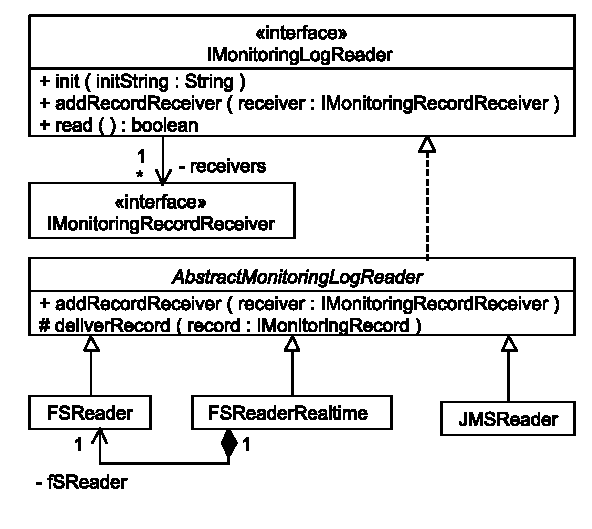
\includegraphics[width=0.5\textwidth]{images/kieker_readerimpls}
\caption{\TODO{update (\method{newMonitoringRecord} method; package names, \ldots)}}
\label{Figure:ReaderHierarchy}
\end{figure}

\noindent The implementation of an own reader is nearly the same as the implementation of the writer, but to keep things simple, it is recommended to extend the already implemented \class{AbstractKiekerMonitoringLogReader}, because otherwise it would be necessary to implement the employed observer pattern of the reader. By using the methods of the abstract class \class{AbstractMonitoringLogReader}, the task of delivering a new record to the consumers can be delegated to the super class.\\
Listing~\ref{listing:MyReader} shows a simple reader which reads a stored record from the pipe. If there is nothing on the pipe to be read, the reader waits 4 seconds at maximum before it terminates.

\setJavaCodeListing
\lstinputlisting[caption=MyPipeReader.java, label=listing:MyReader]{\customComponentsBookstoreApplicationDir/src/bookstoreApplication/MyPipeReader.java}

\section{Analysis Plugins}\label{sec:analysis:plugins}

\TODO{Input/Output ports}

\section{Monitorig Record Consumer Plugins}\label{sec:analysis:consumer}

The consumers are the parts of Kieker which work with the records that have been loaded by the reader. There can be (theoretically) an infinite number of consumers which produce any kind of output. A consumer can be programmed by implementing the interface \class{kieker.analysis.plugin.IMonitoringRecordConsumerPlugin} and writing the necessary methods. Following example consumer takes the given record and writes the content to the default output stream.

\setJavaCodeListing
\lstinputlisting[caption=MyReponseTimeConsumer.java]{\customComponentsBookstoreApplicationDir/src/bookstoreApplication/MyResponseTimeConsumer.java}
